% ######################################################################################################################
%         Clustering
% ######################################################################################################################

\chapter{Clustering}
\label{ch:Clustering}

\paperbox{
    This chapter is based on the peer-reviewed publication:
}{\paperpppp}{
    \textbf{Contributions:} Lucas Czech... Alexandros Stamatakis...
}

% \todo{distance measures, nhd, simulations, mantel test}

% ######################################################################################################################
%         Background and Motivation
% ######################################################################################################################

\section{Background and Motivation}
\label{ch:Clustering:sec:Motivation}

Given a set of metagenomic sequence samples (see \secref{ch:Foundations:sec:SequenceAnalysis:sub:Metagenomics}),
and a distance measure between them (\secref{ch:Foundations:sec:PhylogeneticPlacement:sub:Distances}),
a fundamental task consists in clustering samples that are similar to each other.
For example, Squash Clustering performs agglomerative hierarchical clustering of samples,
as introduced in \secref{ch:Foundations:sec:PhylogeneticPlacement:sub:ExistingMethods:par:SquashClustering}.
It is based on the phylogenetic placement of the \acfp{QS} of the samples on a \acf{RT},
and employs the KR distance to assess sample similarity.
An example of the resulting clustering tree is shown in \figref{fig:squash_edgepca:sub:squash}.

For large datasets, producing a clustering tree can however considered to be a downside of Squash Clustering,
as the number of tips in this tree is equal to the number $n$ of samples that are being clustered.
Thus, for datasets with more than a few hundred samples,
the clustering result becomes hard to inspect and interpret visually.

\begin{figure}[!htb]
    \centering
    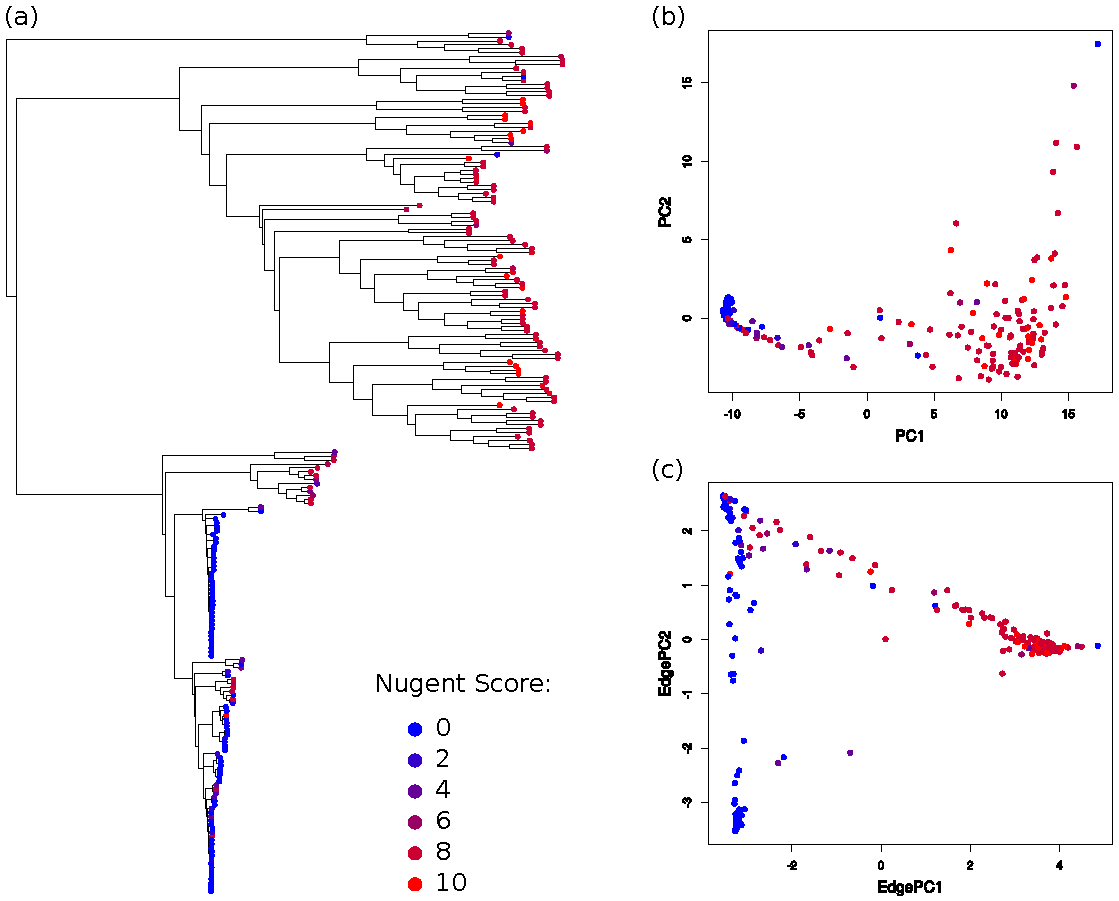
\includegraphics[width=\linewidth]{squash_edgepca.pdf}
    \begin{subfigure}{0pt}
        \phantomcaption
        \label{fig:squash_edgepca:sub:squash}
    \end{subfigure}
    \begin{subfigure}{0pt}
        \phantomcaption
        \label{fig:squash_edgepca:sub:pca}
    \end{subfigure}
    \begin{subfigure}{0pt}
        \phantomcaption
        \label{fig:squash_edgepca:sub:epca}
    \end{subfigure}
    \caption[Existing analysis methods on the BV dataset]{
        \textbf{Existing analysis methods on the BV dataset.}
        We applied \subref{fig:squash_edgepca:sub:squash} Squash Clustering,
        \subref{fig:squash_edgepca:sub:pca} PCA on the pairwise KR distance matrix between samples,
        and \subref{fig:squash_edgepca:sub:epca} Edge PCA,
        using the \acf{BV} dataset \cite{Srinivasan2012}.
        The Subfigures are recalculations of Figure~1(A) of \cite{Srinivasan2012},
        and Figures~4 and 3 of \cite{Matsen2011b}, respectively.
        All Subfigures represent samples as colored dots according to their respective Nugent score,
        which indicates the severeness of the \ac{BV} infection of the samples/patients.
%         In \subref{fig:squash_edgepca:sub:squash}, we added coloring to the samples (tips) of the cluster tree for convenience.
        See \secref{ch:Foundations:sec:PhylogeneticPlacement:sub:ExistingMethods} for a description of the methods,
        and \appref{supp:sec:DetailsEmpiricalDatasets:sub:BV} for details on the dataset.
    }
    \label{fig:squash_edgepca}
\end{figure}

Furthermore, depending on the data and research question at hand,
the KR distance is not always the best measure of sample similarity.
As explained in \secref{ch:Foundations:sec:PhylogeneticPlacement:sub:PlacementProcessing},
edge imbalances can often reveal more subtle differences between samples than edge masses.
Thus, for some datasets, it might make sense to use a distance based on edge imbalances instead.

To further illustrate this, \figref{fig:squash_edgepca:sub:pca} shows
the result of a standard principal component analysis (PCA) \cite{Pearson1901,Jolliffe2002}
on the pairwise KR distance matrix of the \acf{BV} dataset \cite{Srinivasan2012} that we used before.
On the left hand side of the figure, the blue samples,
representing healthy women with a low Nugent score, form a dense cluster.
Towards the right hand side however, the red samples, which belong to sick patients, are spread over the rest of the graph.
As Squash Clustering also uses the KR distance, the same pattern can be observed in its resulting clustering tree,
as shown in \figref{fig:squash_edgepca:sub:squash}:
The bottom half of the clustering tree, containing mainly healthy (blue) samples, has short branches,
which correspond to the dense blue region in \figref{fig:squash_edgepca:sub:pca}.
At the same time, the top half, with mostly samples from sick (red) patients, has many long branches,
corresponding to the scattered red region in \figref{fig:squash_edgepca:sub:pca}.
Thus, Squash Clustering represents equivalent information to a standard PCA on this dataset.
It thus ``suffers'' from the same shortcomings that Edge PCA is solving by using mass imbalance instead
(see \secref{ch:Foundations:sec:PhylogeneticPlacement:sub:ExistingMethods:par:EdgePCA}).
This can be seen in \figref{fig:squash_edgepca:sub:epca}, which shows the result of Edge PCA on the dataset.
There, the healthy (blue) samples clearly separate
into two groups for the two dominant \taxonname{Lactobacillus} clades in healthy patients,
which is due to the edge imbalances resolving smaller differences between the placements on nearby clades in this dataset.
Hence, for this dataset, instead of using a distance based on edge masses such as the KR distance,
edge imbalances should be used to measure distances between samples.

% ######################################################################################################################
%         Methods and Implementation
% ######################################################################################################################

\section{Methods and Implementation}
\label{ch:Clustering:sec:Methods}

We here propose two variants of $k$-means clustering \cite{Steinhaus1956,Macqueen1967},
which we call \emph{Phylogenetic $k$-means}, and \emph{Imbalance $k$-means}, respectively.
They are clustering methods for phylogenetic placement of a set of metagenomic sequence samples,
and address the issues described above.
Note that these methods are clustering samples, and not single sequences \cite{Kelley2010}.
Both methods produce a predefined number of clusters, and hence are able to work with arbitrarily large datasets.
Phylogenetic $k$-means uses the KR distance to assess sample similarity, that is, it uses edge masses,
while Imbalance $k$-means uses edge imbalances instead.

The methods take as input a set of $n$ samples, each consisting of their \acfp{QS} placed on a fixed \acf{RT}.
They then assign the samples to $k$ clusters, each represented by a cluster \emph{centroid}
that describes the average placement mass distribution of the samples assigned to it.
We later also discuss how to chose a reasonable value for $k$.

% ======================================================================================================================
%     Phylogenetic k-means
% ======================================================================================================================

% PDF bookmarks do not accept the $k$ math mode, so make it use the letter instead.
\subsection{Phylogenetic \texorpdfstring{$k$-means}{k-means}}
\label{ch:Clustering:sec:Methods:sub:PhylogeneticKmeans}

Phylogenetic $k$-means employs the KR distance (see \secref{ch:Foundations:sec:PhylogeneticPlacement:sub:Distances:par:KR})
and hence yields results that are consistent with the clustering tree of Squash Clustering.
% but it yields a predefined number of $k$ clusters.

% ----------------------------------------------------------------------------------------------------------------------
%     Algorithm
% ----------------------------------------------------------------------------------------------------------------------

\paragraph{Algorithm}
\label{ch:Clustering:sec:Methods:sub:PhylogeneticKmeans:par:Algorithm}

% The underlying idea is to assign each of the $n$ samples to one of $k$ cluster centroids,
% where each centroid represents the average mass distribution of all samples assigned to it.

The input samples and the cluster centroids are of the same data type,
namely, they are mass distributions on a fixed \ac{RT}.
It is thus possible to calculate the KR distances between samples and centroids,
and to calculate their average mass distributions by \emph{squashing},
as described in \secref{ch:Foundations:sec:PhylogeneticPlacement:sub:PlacementProcessing:par:EdgeMasses}.

The objective is then to find an assignment of the $n$ samples into $k$ clusters
that minimizes the total distance between each sample and the cluster centroid it is assigned to,
measured as the KR distance between them.
That is, for $k$ clusters, each represented by a set $A_k$ of samples assigned to it, and its centroid $C_k$,
the objective is to find

\begin{equation}
    \label{ch:Clustering:eq:KmeansObjective}
    \hat{A} ~=~ \argmin_A \sum_{i=1}^{k} \sum_{s \in A_i} \mbox{KR}( s, C_i )
\end{equation}

% Keep in mind that each sample in the assignments $A_k$ and each centroid $C_k$
% are placement mass distributions on the \ac{RT}, between which the KR distance can be calculated.
The optimal solution $\hat{A}$ for the assignment of samples to clusters can be found via a brute-force search.
However, the number of possible assignments of $n$ samples to $k$ clusters
is given by the Stirling partition number $S(n,k)$ \cite{Graham1989a},
which is too large for any realistic dataset.

Hence, our implementation follows the Lloyd-Forgy algorithm \cite{Lloyd1982,Forgy1965},
which is the standard heuristical method to solve the $k$-means problem.
It iteratively improves the assignments $A$ and the centroids $C$ in two alternating steps,
as shown in \algref{algo:kmeans}.

% \todo{maybe remove space later again:}
% \vspace*{1em}
\begin{algorithm}
\caption{Phylogenetic $k$-means}\label{algo:kmeans}
\begin{algorithmic}[1]
    \State initialize $k$ \textit{Centroids}
    \While{not converged}
        \State assign each \textit{Sample} to nearest \textit{Centroid} ($A$)
        \State update \textit{Centroids} as mass averages of their \textit{Samples} ($C$)
    \EndWhile
    \State \textbf{return} \textit{Assignments} $A$ and \textit{Centroids} $C$
\end{algorithmic}
\end{algorithm}

By default, we use the $k$-means++ initialization algorithm \cite{Arthur2007} to obtain an initial set of $k$ centroids.
It works by subsequent random selection of samples to be used as initial centroids,
until $k$ centroids have been selected.
In each step, the probability of selecting a sample is
proportional to its squared distance to the nearest already selected sample.
Hence, centroids are preferably selected that are far away from each other.
An alternative initialization is to select samples as initial clusters entirely at random.
This is however more likely to yield sub-optimal clusterings \cite{Kanungo2003}.

Then, each sample is assigned to its nearest centroid, using the KR distance. %for example the KR or NH distance.
Lastly, the centroids are updated to represent
the average mass distribution of all samples that are currently assigned to them.
This iterative process alternates between improving the assignments and improving the centroids.
Thus, the main difference to normal $k$-means in the $\mathbb{R}^d$ is the use of phylogenetic information:
Instead of euclidean distances on vectors, we use the KR distance,
and instead of averaging vectors to obtain centroids, we use the average mass distribution on the tree.

The process is repeated until it converges,
that is, the cluster assignments do not change any more between subsequent iterations,
or until a maximum number of iterations have been executed.
% The second stopping criterion makes sure that the algorithm terminates even with non-convergent datasets.
This second stopping criterion is added to avoid the super-polynomial worst case running time of $k$-means,
which however almost never occurs in practice \cite{Bottou1995,Arthur2006}.

The result of the algorithm is an assignment of each sample to one of the $k$ clusters.
As the algorithm relies on the KR distance, it clusters samples with similar relative abundances.
The cluster centroids can be visualized as trees with a mass distribution,
analogous to how Squash Clustering visualizes inner nodes of the clustering tree.
That is, each centroid can be represented as the average mass distribution of the samples that were assigned to it.
This allows to inspect the centroids and thus to interpret how the samples were clustered.
% For instance, the diversity and taxonomic assignment of the centroids represents the corresponding sets of samples.
Examples of this are shown in \figref{fig:centroids}.

% ----------------------------------------------------------------------------------------------------------------------
%     Algorithmic Improvements
% ----------------------------------------------------------------------------------------------------------------------

\paragraph{Algorithmic Improvements}
\label{ch:Clustering:sec:Methods:sub:PhylogeneticKmeans:par:AlgorithmicImprovements}

In each assignment step of the algorithm, distances from all $n$ samples to all $k$ centroids are computed,
which has a time complexity of $\mathcal{O}(n \cdot k)$.
In order to accelerate this step, we can apply branch binning
as introduced in \secref{ch:Foundations:sec:PhylogeneticPlacement:sub:PlacementProcessing:par:EdgeMasses}.
For the \ac{BV} dataset, we found that even using just \num{2} bins per edge does not alter the cluster assignments.
Branch binning reduces the number of mass points that have to be accessed in memory during KR distance calculations;
however, the costs for tree traversals remain.
Thus, we observed a maximal speedup of 75\% when using one bin per branch,
see \tabref{tab:hmp_binning_error} for details.
Intermediate binning strategies are also possible:
instead of binning all masses of the input samples, just the centroid masses can be binned.

% even binning to \num{1} bin,
% that is, combining all placement masses on a branch into one point,
% changes the cluster assignment of only \num{2} of {220} samples
% -- both of which were near the border between two clusters.
% The main bottleneck in the computation however seems to be
% the random memory access to the edges and per-edge masses induced by the tree traversals
% so that binning does not yield substantial speedups.
% In our tests, summarizing all masses in one bin per branch resulted in a speedup of around 75\%,

Furthermore, during the execution of the algorithm, empty clusters can occur,
for example, if $k$ is greater than the number of natural clusters in the data.
Although this problem did not occur in our tests, we implemented the following solution:
First, find the cluster with the highest variance.
Then, choose the sample of that cluster that is furthest from its centroid,
and assign it to the empty cluster instead.
This process is repeated if multiple empty clusters occur at once in an iteration.

% ======================================================================================================================
%         Imbalance k-means
% ======================================================================================================================

% PDF bookmarks do not accept the $k$ math mode, so make it use the letter instead.
\subsection{Imbalance \texorpdfstring{$k$-means}{k-means}}
\label{ch:Clustering:sec:Methods:sub:ImbalanceKmeans}

We further propose \emph{Imbalance $k$-means},
which is a variant of $k$-means that makes use of the edge imbalance transformation
(see \secref{ch:Foundations:sec:PhylogeneticPlacement:sub:PlacementProcessing:par:EdgeImbalances}),
and thus takes the clades of the reference tree into account.
In order to quantify the difference in imbalances between two samples,
we use the Euclidean distance between their imbalance vectors (that is, rows of the imbalance matrix).
This is a suitable distance measure,
as the imbalances implicitly capture the tree topology as well as the placement mass distributions.
As a consequence, the expensive tree traversals required for Phylogenetic $k$-means are not necessary for the calculations.
The algorithm takes the edge imbalance matrix of normalized samples as input,
% as shown in \figref{fig:imbalance:sub:Matrices},
and performs a standard Euclidean $k$-means clustering following the Lloyd-Forgy algorithm \cite{Lloyd1982,Forgy1965}.
% As there is no apparent phylogenetically informative distance measure between imbalance vectors,
% we use euclidean distance instead.
% This also allows to calculated centroids as simple vector averages.

This variant of $k$-means tends to find clusters that are consistent with the results of Edge PCA,
as both use the same input data (imbalances) and both operate in Euclidean space. %as well as the same distance measure.
Furthermore, as the method does not need to calculate KR distances,
and thus neither involves tree traversals nor needs to consider each placement location (or bins of those) separately,
it is several orders of magnitude faster than Phylogenetic $k$-means.
For example, on the \ac{HMP} dataset (see \appref{supp:sec:DetailsEmpiricalDatasets:sub:HMP}),
it runs in mere seconds, instead of several hours needed for Phylogenetic $k$-means;
see Section \secref{ch:Clustering:sec:Results:sub:Performance} for details.

% ======================================================================================================================
%     Finding k
% ======================================================================================================================

\subsection{Finding appropriate values for \texorpdfstring{$k$}{k}}
\label{ch:Clustering:sec:Methods:sub:FindingK}

A commonly criticized downside of $k$-means clustering in general is
that the number of clusters $k$ is an input parameter to the algorithm.
Hence, a key question is how to select an appropriate $k$
that reflects the number of ``natural'' clusters in the data.
There exist various suggestions in the literature
\cite{Thorndike1953,Rousseeuw1987,Bischof1999,Pelleg2000,Tibshirani2001,Hamerly2004}.
% See also: https://stackoverflow.com/a/1793572/4184258 and
% http://www.sthda.com/english/articles/29-cluster-validation-essentials/96-determining-the-optimal-number-of-clusters-3-must-know-methods/

We evaluated the Elbow method \cite{Thorndike1953},
which is a straight forward method that yielded reasonable results for our test datasets.
It works by plotting the cluster variance,
that is, the average squared distance of the samples to their assigned cluster centroids,
for different values of $k$.
On the one hand, for low values of $k$, many samples exhibit a large distance to their assigned centroid,
% the distances from samples to their assigned centroids are relatively
inducing a high variance.
On the other hand, higher values of $k$ further split the clusters and hence reduce the variance.
% and slightly reduce this distance by further splitting clusters.
Thus, at a given point, increasing $k$ only yields a marginal change in variance.
If the data has a natural number of clusters, the corresponding $k$ at this point produces an angle in the plot,
called the \emph{elbow}.
Thus, the presence of an elbow in the variance plot indicates reasonable values for $k$.

Additionally, for a quantitative evaluation of the clusterings,
we used the $k$ that arose from the number of distinct categories or labels based on the available meta-data for the data.
% that is, the number of distinct categories our data is known to belong to.
For example, the samples of the \ac{HMP} dataset are labeled with \num{18} distinct body sites,
describing where each sample was taken from, c.f.~\figref{fig:hmp_kmeans_all_18}.

% ######################################################################################################################
%         Results
% ######################################################################################################################

\section{Evaluation and Results}
\label{ch:Clustering:sec:Results}

We here evaluate the two $k$-means variants in terms of their clustering accuracy and performance.
We used the \acf{BV} dataset (see \appref{supp:sec:DetailsEmpiricalDatasets:sub:BV} for details)
as an example of a small dataset to which methods such as Squash Clustering \cite{Matsen2011a}
are still applicable for comparison,
and the \acf{HMP} dataset (see \appref{supp:sec:DetailsEmpiricalDatasets:sub:HMP})
to showcase that our methods scale to datasets that are too large for existing methods.

% ======================================================================================================================
%     BV Dataset
% ======================================================================================================================

\subsection{BV Dataset}
\label{ch:Clustering:sec:Results:sub:BVDataset}

We placed the samples of the \ac{BV} dataset \cite{Srinivasan2012}
on the re-inferred reference tree of their original reference sequences
to test whether our methods work as expected.
To this end, we ran both Phylogenetic $k$-means and Imbalance $k$-means on the \ac{BV} dataset,
and compare the results to the existing analysis of the data in \cite{Srinivasan2012} and \cite{Matsen2011a}.
We chose $k:=3$, inspired by the findings of \cite{Srinivasan2012}.
There, they distinguish between subjects affected by Bacterial Vaginosis and healthy subjects,
and further separate the healthy ones into two categories depending on the dominating clade in the vaginal microbiome,
which is either \taxonname{Lactobacillus iners} or \taxonname{Lactobacillus crispatus}.
Any choice of $k > 3$ would simply result in smaller, more fine-grained clusters,
but not change the general findings of these experiments.
The number of clusters is also evaluated using the Elbow method later in \secref{ch:Clustering:sec:Results:sub:ElbowMethod}.

For each of the \num{220} samples of the dataset, we hence obtained two cluster assignments:
First, by using Phylogenetic $k$-means, we obtained the cluster assignment \emph{PKM}.
Second, by using Imbalance $k$-means, we obtained assignment \emph{IKM}.
In the following figures, the samples are represented by colored circles:
red, green, and blue show the cluster assignments \emph{PKM},
while purple, orange, and gray show the cluster assignments \emph{IKM}.
We use two different color sets for the two methods, in order to make them distinguishable at first glance.
Note that the mapping of colors to clusters is arbitrary and depends on the random initialization of the algorithm.

We then conducted Squash Clustering and Edge PCA (\secref{ch:Foundations:sec:PhylogeneticPlacement:sub:ExistingMethods})
on the dataset, thereby reproducing results of previous studies,
as well as two alternative dimensionality reduction methods.
This allows for a direct comparison between our novel and the existing methods.

% The figure shows the results of Squash Clustering, Edge PCA, and two alternative dimensionality reduction methods,
% colorized by the cluster assignments \emph{PKM} of Phylogenetic $k$-means (in red, green, and blue)
% and \emph{IKM} of the Imbalance $k$-means (in purple, orange, and gray), respectively.

% ----------------------------------------------------------------------------------------------------------------------
%     Squash Clustering
% ----------------------------------------------------------------------------------------------------------------------

\paragraph{Comparison to Squash Clustering}
\label{ch:Clustering:sec:Results:sub:BVDataset:par:SquashClustering}

\begin{figure}[p]
    \centering
    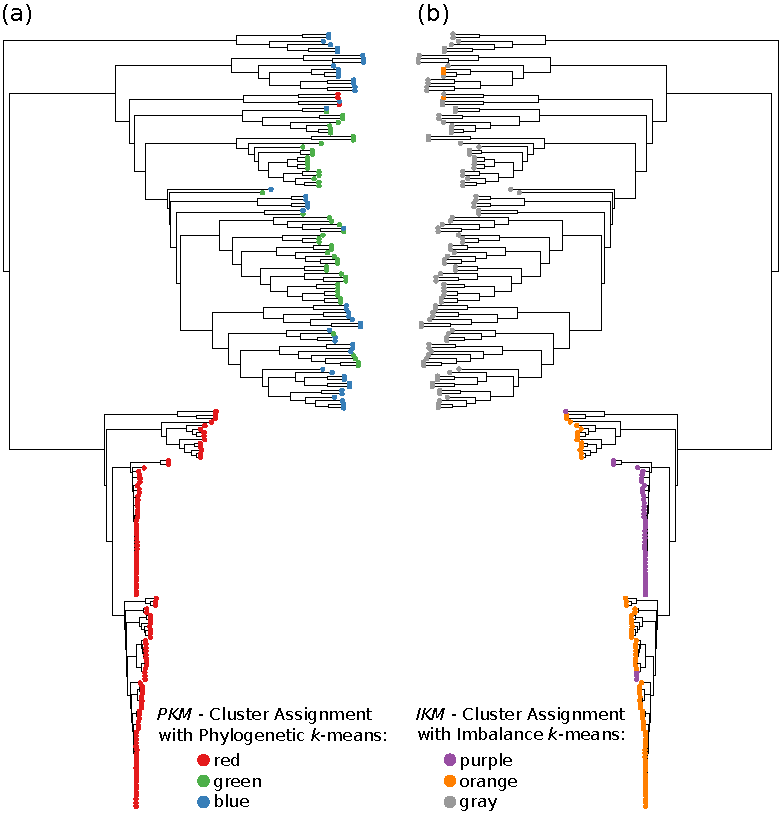
\includegraphics[width=\linewidth]{cluster_kmeans_trees.pdf}
    \begin{subfigure}{0pt}
        \phantomcaption
        \label{fig:cluster_kmeans_trees:sub:mass_tree}
    \end{subfigure}
    \begin{subfigure}{0pt}
        \phantomcaption
        \label{fig:cluster_kmeans_trees:sub:imbalance_tree}
    \end{subfigure}
    \caption[Comparison of $k$-means clustering to Squash Clustering]{
        \textbf{Comparison of $k$-means clustering to Squash Clustering.}
        We applied Squash Clustering to the \ac{BV} dataset \cite{Srinivasan2012},
        to compare it to the assignments obtained from our $k$-means variants.
        % in order to compare them to existing methods.
%         See \cite{Srinivasan2012} for details of the dataset and its interpretation.
%         We chose $k:=3$, as this best fits the features of the dataset.
        % Sub (A)
        \subref{fig:cluster_kmeans_trees:sub:mass_tree}
        Hierarchical cluster tree of the samples, using Squash Clustering.
        The tree is a recalculation of Figure~1(A) of \cite{Srinivasan2012}.
        Each leaf represents a sample; branch lengths are KR distances.
        We added color coding for the samples, using \emph{PKM}.
        The lower half of red samples are mostly healthy subjects,
        while the green and blue upper half are patients affected by Bacterial Vaginosis.
        % Sub (B)
        \subref{fig:cluster_kmeans_trees:sub:imbalance_tree}
        The same tree, but annotated by \emph{IKM}.
        The tree is flipped horizontally for ease of comparison.
        The healthy subjects are split into two sub-classes,
        discriminated by the dominating species in their vaginal microbiome:
        orange and purple represent samples were \taxonname{Lactobacillus iners} and \taxonname{Lactobacillus crispatus}
        dominate the microbiome, respectively.
        The patients mostly affected by BV are clustered in gray.
    }
    \label{fig:cluster_kmeans_trees}
\end{figure}

The comparison of our $k$-means clustering assignments to Squash Clustering is shown in \figref{fig:cluster_kmeans_trees}.
As can be seen in \figref{fig:cluster_kmeans_trees:sub:mass_tree}, Squash Clustering as well as
Phylogenetic $k$-means can distinguish healthy subjects from those affected by Bacterial Vaginosis.
Healthy subjects constitute the lower part of the cluster tree.
They have shorter branches between each other, indicating the smaller KR distance between them,
which is a result of the dominance of \taxonname{Lactobacillus} in healthy subjects.
The same clusters are found by Phylogenetic $k$-means:
As it uses the KR distance, it assigns all healthy subjects to one cluster (shown in red),
which is consistent with the short cluster tree branches in \figref{fig:cluster_kmeans_trees:sub:mass_tree}.
The green and blue clusters are mostly the subjects affected by the disease.

In \figref{fig:cluster_kmeans_trees:sub:imbalance_tree}, we compare Squash Clustering to Imbalance $k$-means.
Here, the distinction between the two \taxonname{Lactobacillus} clades
can be seen by the purple and orange cluster assignments.
The cluster tree also separates those clusters into two clades.
The separate small group of orange samples above the purple clade is an artifact of the tree visualization (ladderization),
and actually is close to the other orange samples below.
The diseased subjects are all assigned to the gray cluster, represented by the upper half of the cluster tree.
It is apparent that both methods separate the same samples from each other.

% ----------------------------------------------------------------------------------------------------------------------
%     Edge PCA
% ----------------------------------------------------------------------------------------------------------------------

\paragraph{Comparison to Edge PCA}
\label{ch:Clustering:sec:Results:sub:BVDataset:par:EdgePCA}

\begin{figure}[p]
    \centering
    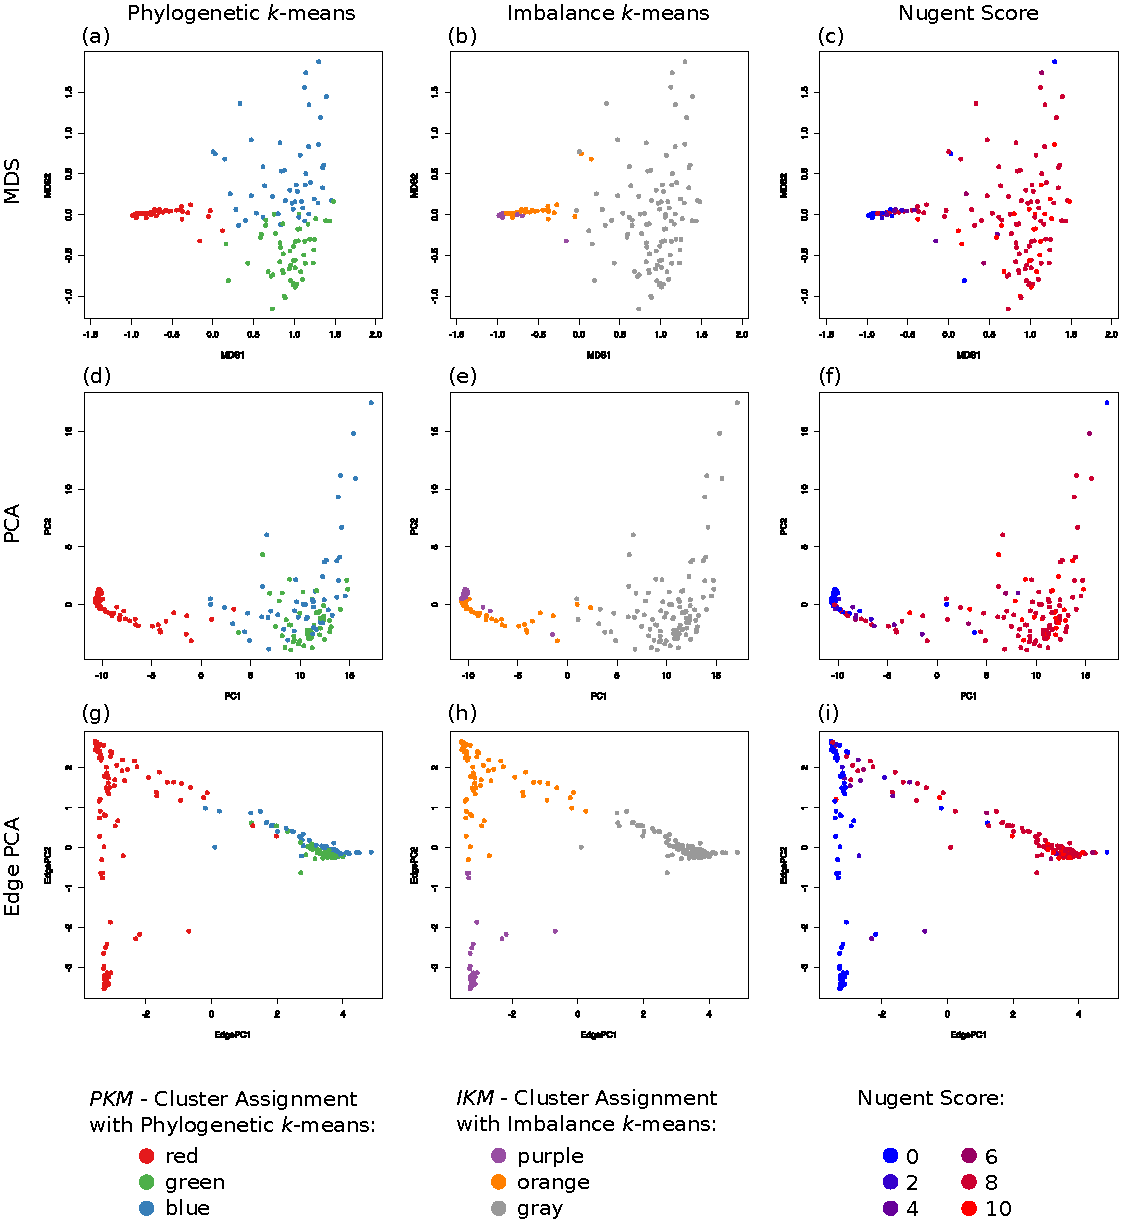
\includegraphics[width=\linewidth]{kmeans_all.pdf}
    \begin{subfigure}{0pt}
        \phantomcaption
        \label{fig:kmeans_all:sub:mds_em}
    \end{subfigure}
    \begin{subfigure}{0pt}
        \phantomcaption
        \label{fig:kmeans_all:sub:mds_ei}
    \end{subfigure}
    \begin{subfigure}{0pt}
        \phantomcaption
        \label{fig:kmeans_all:sub:mds_ns}
    \end{subfigure}
    \begin{subfigure}{0pt}
        \phantomcaption
        \label{fig:kmeans_all:sub:pca_em}
    \end{subfigure}
    \begin{subfigure}{0pt}
        \phantomcaption
        \label{fig:kmeans_all:sub:pca_ei}
    \end{subfigure}
    \begin{subfigure}{0pt}
        \phantomcaption
        \label{fig:kmeans_all:sub:pca_ns}
    \end{subfigure}
    \begin{subfigure}{0pt}
        \phantomcaption
        \label{fig:kmeans_all:sub:epca_em}
    \end{subfigure}
    \begin{subfigure}{0pt}
        \phantomcaption
        \label{fig:kmeans_all:sub:epca_ei}
    \end{subfigure}
    \begin{subfigure}{0pt}
        \phantomcaption
        \label{fig:kmeans_all:sub:epca_ns}
    \end{subfigure}
    \caption[Comparison of $k$-means clustering to MDS, PCA, and Edge PCA]{
        \textbf{Comparison of $k$-means clustering to MDS, PCA, and Edge PCA.}
        Here, we show the dimensionality reduction methods MDS, PCA, and Edge PCA (one per row) on the \ac{BV} dataset.
        MDS and PCA were calculated on the pairwise KR distance matrix of the samples,
        Edge PCA was calculated using the placements on the re-inferred \ac{RT} of the original publication \cite{Srinivasan2012}.
        The plots are colored by the cluster assignments \emph{PKM} and \emph{IKM}
        as found by our $k$-means variants (first two columns), and by the Nugent score of the samples (third column).
        The Nugent score is included to allow comparison of the health status of patients with the clustering results.
        \subref{fig:kmeans_all:sub:pca_ns} and \subref{fig:kmeans_all:sub:epca_ns} are recalculations of
        Figures~4 and 3 of \cite{Matsen2011b}, respectively.
    }
    \label{fig:kmeans_all}
\end{figure}

In \figref{fig:kmeans_all}, we compare the assignments obtained from our $k$-means variants
to several dimensionality reduction methods, such as Edge PCA.
The figure reveals additional details about how the $k$-means method works,
that is, which samples are assigned to the same cluster.

The first row of \figref{fig:kmeans_all} shows the result of
\acf{MDS} of the pairwise KR distance matrix between the samples.
\ac{MDS} \cite{Mardia1978,Krzanowski1994,Everitt2010} is a dimensionality reduction method that
can be used for visualizing levels of similarity between data points.
Given a pairwise distance matrix, it finds an embedding into lower dimensions (in this case, \num{2} dimensions)
that preserves higher dimensional distances as well as possible.

The distinguishing features between the green and the blue cluster
are not apparent in the Squash cluster tree in \figref{fig:cluster_kmeans_trees:sub:mass_tree}.
This can however be seen in \figref{fig:kmeans_all:sub:mds_em}, which shows the \ac{MDS} plot colored by \emph{PKM}.
Here, the red cluster forms a dense region, which is in agreement with the short branch lengths
in the cluster tree of \figref{fig:cluster_kmeans_trees:sub:mass_tree}.
At the same time, the green and blue cluster are separated in the \ac{MDS} plot,
but form a coherent region of low density,
indicating that $k:=3$ might be too large when applying Phylogenetic $k$-means to this dataset.
That is, the actual clustering just distinguishes healthy from sick patients (c.\,f.~\figref{fig:elbows}),
meaning that \num{2} dimensions might also suffice here.
% which, albeit not well separated from each other, indicate groups of samples with lower KR distance between each other.
Although the separation between green and blue samples is smooth,
it shows that Phylogenetic $k$-means finds clusters based on KR distance between samples,
and thus yields results consistent with Squash Clustering and \ac{MDS}.

A similar visualization of the pairwise KR distances is shown in the second row of \figref{fig:kmeans_all},
where we applied standard \acf{PCA} \cite{Krzanowski1994,Everitt2010} to the pairwise KR distance matrix
by interpreting it as a data matrix.
Although it is mathematically sound, the direct application of \ac{PCA} to a distance matrix lacks a simple interpretation,
which was previously used to motivate Edge PCA
(c.\,f.~\secref{ch:Foundations:sec:PhylogeneticPlacement:sub:ExistingMethods:par:EdgePCA}).
Still, this can be seen as a visualization of the distances that helps understanding our methods.

For example, in \figref{fig:kmeans_all:sub:pca_em},
% It is a recalculation of Figure~4 in the preprint \cite{Matsen2011b},
% which did not appear in the final published version \cite{Matsen2011a}.
% It is a recalculation of Figure~4 of \cite{Matsen2011b}.
% but can also be found at \cite{MatsenEdgePCA}.
which shows the PCA plot colored by \emph{PKM}, the red cluster again is clearly separated from the rest.
This time however, the distinction between the green and the blue cluster
is not as apparent as in \figref{fig:kmeans_all:sub:mds_em}.

Furthermore, \figref{fig:kmeans_all:sub:mds_ei} and \subref{fig:kmeans_all:sub:pca_ei} show the MDS and the PCA plot,
respectively, this time colored by \emph{IKM}.
Here, the purple cluster found by Imbalance $k$-means forms a dense cluster of close-by samples on the left of the plots,
which is in accordance with the short branch lengths
of this cluster as shown in the clustering tree in \figref{fig:cluster_kmeans_trees:sub:imbalance_tree}.
The orange cluster is slightly more spread out in the plots,
which again can be seen by the longer branch lengths in \figref{fig:cluster_kmeans_trees:sub:imbalance_tree}.

Finally, we applied Edge PCA to the samples, as shown in the last row of \figref{fig:kmeans_all}.
In particular, \figref{fig:kmeans_all:sub:epca_ei} compares Imbalance $k$-means to Edge PCA
by coloring the plot using \emph{IKM}.
% The plot is a recalculation of Figure~3 of \cite{Matsen2011b}, which also appeared in Figure~6 in \cite{Matsen2011a}
% and Figure~3 in \cite{Srinivasan2012},
Because both methods work on edge imbalances, they group the data in the same way, and are thus consistent with each other.
That is, they clearly separate the two healthy groups and the diseased one from each other.
Edge PCA forms a plot with three corners, which are colored by the three Imbalance $k$-means cluster assignments.

% ----------------------------------------------------------------------------------------------------------------------
%     Cluster Centroids
% ----------------------------------------------------------------------------------------------------------------------

\paragraph{Cluster Centroids}
\label{ch:Clustering:sec:Results:sub:BVDataset:par:ClusterCentroids}

As mentioned before, an advantage of using phylogenetic placements as input to our $k$-means clustering methods
is the ability to visualize cluster centroids by showing the average mass distribution
of the samples assigned to them on the underlying \acf{RT}.
In Phylogenetic $k$-means, the mass distributions of the centroids are already part of the algorithm,
as they are needed for calculating the KR distances between samples and centroids.
In Imbalance $k$-means however, the placement data is used in form of edge imbalances instead of masses.
Still, after convergence of the algorithm, the per-centroid average mass can be calculated from the input samples
and again visualized on the \ac{RT}.

\begin{figure}[!tb]
    \centering
    \includegraphics[width=\linewidth]{centroids.pdf}
    \begin{subfigure}{0pt}
        \phantomcaption
        \label{fig:centroids:sub:red}
    \end{subfigure}
    \begin{subfigure}{0pt}
        \phantomcaption
        \label{fig:centroids:sub:green}
    \end{subfigure}
    \begin{subfigure}{0pt}
        \phantomcaption
        \label{fig:centroids:sub:blue}
    \end{subfigure}
    \begin{subfigure}{0pt}
        \phantomcaption
        \label{fig:centroids:sub:purple}
    \end{subfigure}
    \begin{subfigure}{0pt}
        \phantomcaption
        \label{fig:centroids:sub:orange}
    \end{subfigure}
    \begin{subfigure}{0pt}
        \phantomcaption
        \label{fig:centroids:sub:gray}
    \end{subfigure}
    \caption[Example of $k$-means cluster centroids visualization]{
        % In this figure, I assume that the reader is already familiar with the characteristics of the dataset.
        % No need to repeat everything over again...
        \textbf{Example of $k$-means cluster centroids visualization.}
        Here we show the cluster centroids as found by our $k$-means variants using the \ac{BV} dataset,
        visualized on the reference tree via color coding.
        The cluster assignments are the same as in \figref{fig:cluster_kmeans_trees} and \figref{fig:kmeans_all};
        the first row show the three clusters found by Phylogenetic $k$-means,
        the second row the clusters found by Imbalance $k$-means.
        Each tree represents one centroid around which the samples were clustered,
        that is, it shows the combined masses of the samples that were assigned to that cluster.
        The edges are colored relative to each other, using a linear scaling of
        light blue (no mass), purple (half of the maximal mass) and black (maximal mass).
        The two \taxonname{Lactobacillus} clades are marked with black arcs on the left of the trees.
    }
    \label{fig:centroids}
\end{figure}

Examples of this are shown in \figref{fig:centroids},
for both sample assignments \emph{PKM} (first row) and \emph{IKM} (second row) of the \ac{BV} dataset.
As explained above, the samples can be split into three groups:
The diseased subjects, which have placement mass in various parts of the tree,
as well as two groups of healthy subjects, with placement mass in one of two \taxonname{Lactobacillus} clades,
marked with black arcs in \figref{fig:centroids}.
This grouping is also clearly visible in the trees.
The red cluster in \subref{fig:centroids:sub:red} for example represents all healthy subjects;
thus, most of its mass is located in the two \taxonname{Lactobacillus} clades.
The purple and orange clusters in \subref{fig:centroids:sub:purple} and \subref{fig:centroids:sub:orange}
on the other hand show a difference in placement mass between those clades.
Furthermore, the placement mass of the gray cluster in \subref{fig:centroids:sub:gray} is mostly
a combination of the masses of the green and blue cluster in \subref{fig:centroids:sub:green} and \subref{fig:centroids:sub:blue},
all of which represent diseased subjects.
These observations are in accordance with the previous findings above,
and further support that our methods yield results that are in agreement with existing methods.
% In summary, our novel $k$-means variants find clusters that are in agreement with existing methods.

% ======================================================================================================================
%     HMP Dataset
% ======================================================================================================================

\subsection{HMP Dataset}
\label{ch:Clustering:sec:Results:sub:HMPDataset}

The \acf{HMP} dataset \cite{Huttenhower2012,Methe2012} (see \appref{supp:sec:DetailsEmpiricalDatasets:sub:HMP} for details)
is used here as an example to show that our method scales to large datasets.
To this end, we used the unconstrained \taxonname{Bacteria} \ac{RT} with \num{1 914} taxa
obtained from our \ac{PhAT} method, see \secref{ch:AutomaticTrees:sec:Evaluation:sub:ReferenceTreeSetup} for details.
% as provided by our Automatic Reference Tree method \cite{Czech2018}.
The tree represents a broad taxonomic range of \taxonname{Bacteria},
that is, the sequences were \emph{not} explicitly selected for the \ac{HMP} dataset,
in order to test the robustness of our clustering methods.
We then placed the \num{9 192} samples of the \ac{HMP} dataset with a total of \num{118 701 818} sequences on that tree,
and calculated Phylogenetic and Imbalance $k$-means on the samples.

The freely available meta-data for the \ac{HMP} dataset labels each sample by the body site were it was taken from.
As there are \num{18} different body site labels, we used $k:=18$.
The resulting clustering assignments are shown in \figref{fig:hmp_kmeans_all_18}.
Furthermore, in \figref{fig:hmp_kmeans_all_8},
we show a clustering of this dataset into $k:=8$ broader body site groups
to exemplify the effect of using different values of $k$.
See \tabref{tab:hmp_data_overview} for the grouping of the original body site labels.
The effect of $k$ on the clustering results is further explored by using the Elbow method,
as described later in \secref{ch:Clustering:sec:Results:sub:ElbowMethod}.
% that is, using the constrained Bacterial tree as well as Imbalance $k$-means.

\begin{figure}[hpbt]
    \centering
    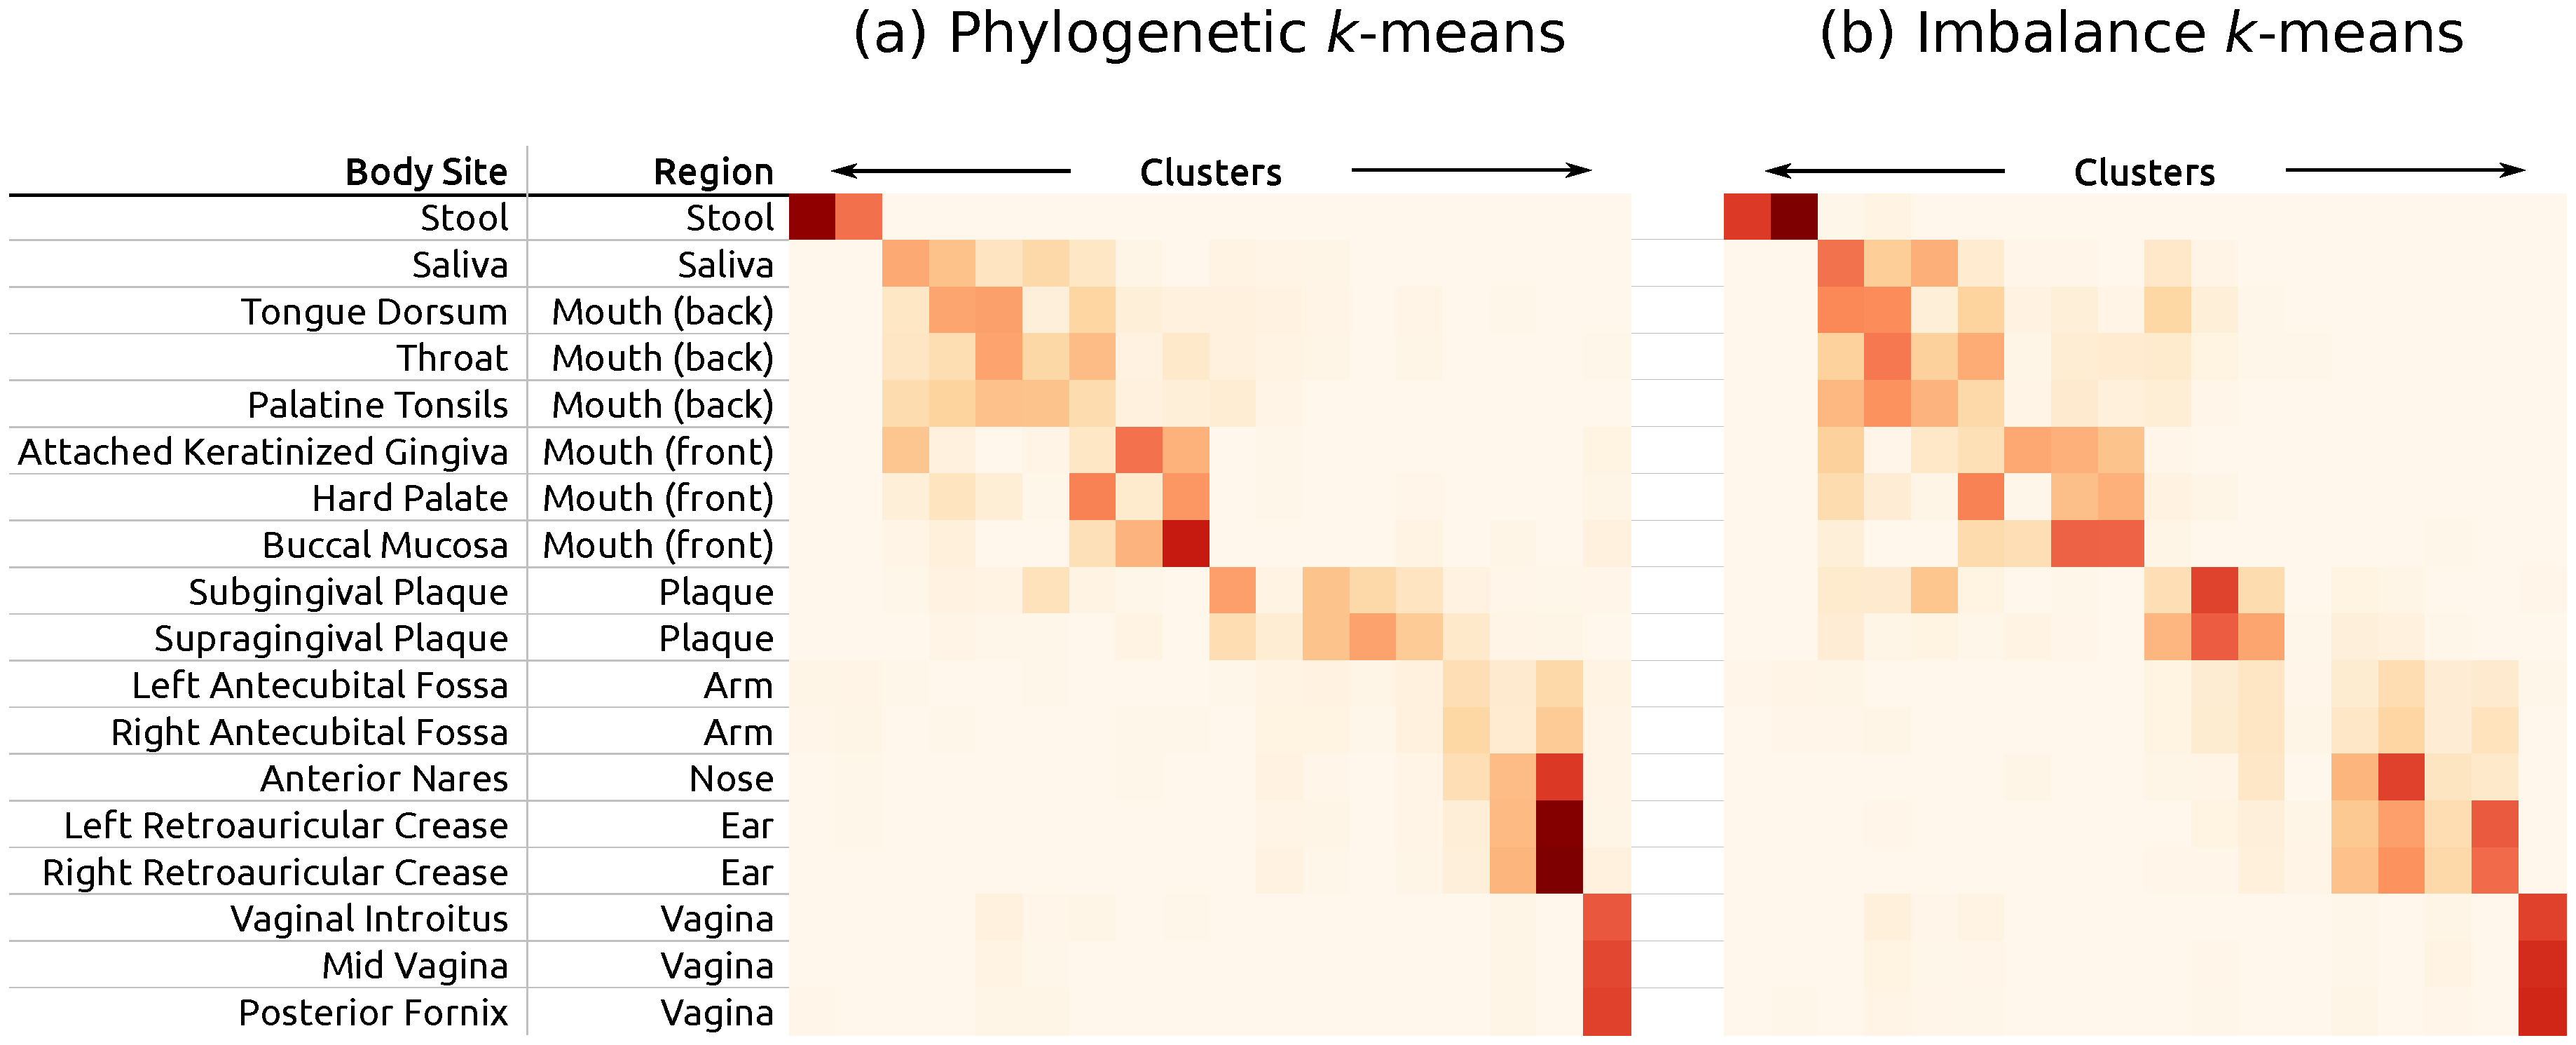
\includegraphics[width=\linewidth]{hmp_kmeans_all_18.pdf}
    \begin{subfigure}{0pt}
        \phantomcaption
        \label{fig:hmp_kmeans_all_18:sub:em_unconstr}
    \end{subfigure}
    \begin{subfigure}{0pt}
        \phantomcaption
        \label{fig:hmp_kmeans_all_18:sub:ei_unconstr}
    \end{subfigure}
    \caption[$k$-means cluster assignments of the \acs{HMP} dataset with $k:=18$]{
        \textbf{$k$-means cluster assignments of the \acs{HMP} dataset with $k:=18$.}
        Here, we show the cluster assignments as yielded by
        \subref{fig:hmp_kmeans_all_18:sub:em_unconstr} Phylogenetic $k$-means and
        \subref{fig:hmp_kmeans_all_18:sub:ei_unconstr} Imbalance $k$-means on the \ac{HMP} dataset.
        We used $k:=18$, which is the number of body site labels in the dataset,
        in order to compare the clusterings to this ``ground truth''.
        Each row represents a body site; each column one of the 18 clusters found by the algorithm.
        We also show a translation of the body site labels into the corresponding body regions.
        The color values indicate how many samples of a body site are assigned to each cluster.
        Similar body sites are clearly grouped together in coherent blocks, indicated by darker colors.
        For example, the stool samples are split into two clusters (topmost row),
        while the three vaginal sites are all put into one cluster (rightmost column).
        However, the algorithm cannot always distinguish between nearby body sites,
        as can be seen from the fuzziness of the clusters of oral samples.
%         Lastly, the figure also lists how the body site labels were aggregated into coarse regions
%         as used in \figref{fig:hmp_kmeans_all_8}.
    }
    \label{fig:hmp_kmeans_all_18}
\end{figure}

\begin{figure}[hpbt]
    \centering
    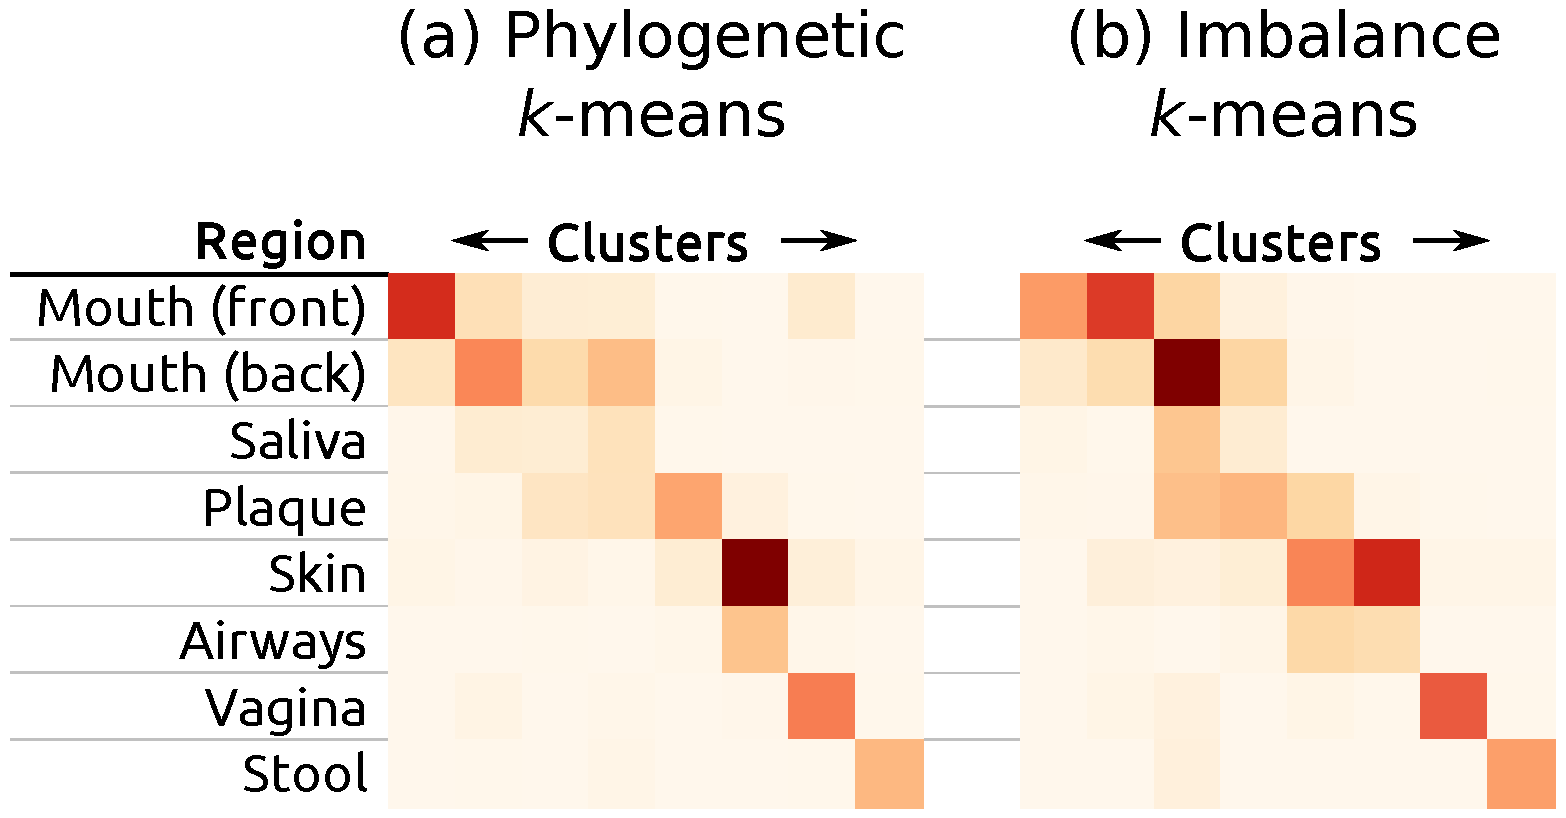
\includegraphics[width=0.6\linewidth]{hmp_kmeans_all_8.pdf}
    \begin{subfigure}{0pt}
        \phantomcaption
        \label{fig:hmp_kmeans_all_8:sub:em_unconstr}
    \end{subfigure}
    \begin{subfigure}{0pt}
        \phantomcaption
        \label{fig:hmp_kmeans_all_8:sub:ei_unconstr}
    \end{subfigure}
    \caption[$k$-means cluster assignments of the \acs{HMP} dataset with $k:=8$]{
        \textbf{$k$-means cluster assignments of the \acs{HMP} dataset with $k:=8$.}
        Here, we again show the cluster assignments as yielded by
        \subref{fig:hmp_kmeans_all_8:sub:em_unconstr} Phylogenetic $k$-means and
        \subref{fig:hmp_kmeans_all_8:sub:ei_unconstr} Imbalance $k$-means on the \ac{HMP} dataset,
        but with $k$ being set to 8, instead of $k:=18$ as in \figref{fig:hmp_kmeans_all_18}.
        These \num{8} clusters are based on an aggregation of the original body site labels into groups,
        as shown in \tabref{tab:hmp_data_overview}.
%         for the list of how the original body site labels were aggregated.
        %for the cluster assignment where $k$ is set to the original number of labels;
        Each row represents a body group; each column one of the \num{8} clusters found by the algorithm.
%         The color values indicate how many samples of a body site were assigned to each cluster.
        Some of the body sites are again clearly separated,
        while particularly the samples from the oral region are distributed over different clusters.
%         This might be due to %the broad reference tree not being able to resolve the fine details between these samples,
%         but might also indicate a
%         homogeneity of the oral samples.
    }
    \label{fig:hmp_kmeans_all_8}
\end{figure}

% Ideally, each cluster would contain only samples from the same body site.
Ideally, all samples from one body site would be assigned to the same cluster,
hence forming a diagonal in the plots of \figref{fig:hmp_kmeans_all_18} and \figref{fig:hmp_kmeans_all_8}.
However, as there are several nearby body sites, which share a large fraction of their microbiome \cite{Huttenhower2012},
we do not expect a perfect clustering.
Furthermore, we used a broad reference tree that might not be able to resolve details in some clades.
% which was originally meant only for a first classification of sequences (see above).
% Thus, the tree does not particularly suit the dataset well.
Nonetheless, the clustering is reasonable, which indicates a robustness against the exact choice of reference taxa.
% and can thus be used for distinguishing among samples.

The plots of the two $k$-means variants generally exhibit similar characteristics in \figref{fig:hmp_kmeans_all_18}.
Most prominently, the stool and vaginal samples are clearly clustered into coherent blocks in both variants.
There are however also some differences.
For example, the samples from the body surface (arm, nose, and ear)
form two relatively dense clusters (columns) in \figref{fig:hmp_kmeans_all_18:sub:em_unconstr},
whereas those sites are spread across four or five clusters in \figref{fig:hmp_kmeans_all_18:sub:ei_unconstr}.
% In general however, these samples form two blocks of cluster columns in both plots.
On the other hand, the mouth samples are more densely clustered in \figref{fig:hmp_kmeans_all_18:sub:ei_unconstr}.

It is remarkable that the oral samples are mostly split into two blocks,
corresponding to the front of the mouth and its back, in both variants of $k$-means in \figref{fig:hmp_kmeans_all_18}.
This indicates that the clustering is sensitive to such subtle differences.
However, within these blocks, there is some fuzziness in the clustering.
This might be caused by our broad reference tree,
and could potentially be resolved by using a tree more specialized for the data/region.
It could however also simply be an artifact of the homogeneity of samples
taken from the close-by oral regions of the human body.

Lastly, using the two \taxonname{General} trees of our \ac{PhAT} method
as described in \secref{ch:AutomaticTrees:sec:Evaluation:sub:ReferenceTreeSetup},
we again evaluated the cluster assignments on the \ac{HMP} datasets (data not shown).
Using this even less specific set of reference taxa yielded cluster assignments
which are almost identical to the ones shown above, except for slightly more fuzziness.
We thus expect that the clustering improves when using an \ac{RT}
containing taxa specifically chosen for the type of sequences in the dataset.
% This however remains future work.

% ======================================================================================================================
%     k-means Elbow Plots
% ======================================================================================================================

\subsection{Elbow Method}
\label{ch:Clustering:sec:Results:sub:ElbowMethod}

As explained in \secref{ch:Clustering:sec:Methods:sub:FindingK},
plots of the cluster variance can be used for the Elbow method
in order to find an appropriate number of clusters in a dataset \cite{Thorndike1953}.
\figref{fig:elbows} shows these plots for our two test datasets.

\begin{figure}[hpbt!]
    \centering
    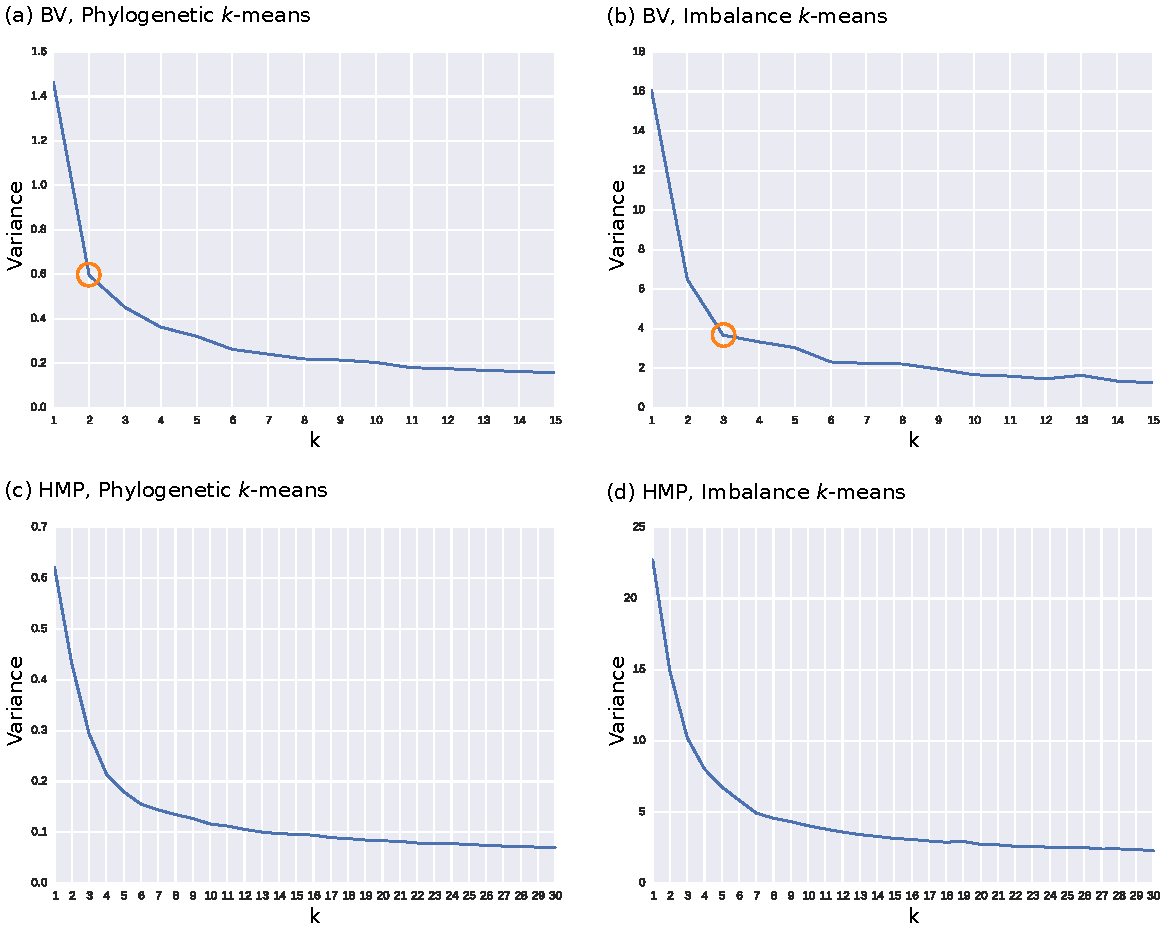
\includegraphics[width=\linewidth]{elbows.pdf}
    \begin{subfigure}{0pt}
        \phantomcaption
        \label{fig:elbows:sub:bv_phylo}
    \end{subfigure}
    \begin{subfigure}{0pt}
        \phantomcaption
        \label{fig:elbows:sub:bv_imb}
    \end{subfigure}
    \begin{subfigure}{0pt}
        \phantomcaption
        \label{fig:elbows:sub:hmp_phylo}
    \end{subfigure}
    \begin{subfigure}{0pt}
        \phantomcaption
        \label{fig:elbows:sub:hmp_imb}
    \end{subfigure}
    \caption[Variances of $k$-means clusters in our test datasets]{
        \textbf{Variances of $k$-means clusters in our test datasets.}
        The figures show the cluster variance for different values of $k$.
        The first row are clusterings of the BV dataset, the second row of the HMP dataset.
        They were clustered using Phylogenetic $k$-means (first column),
        and Imbalance $k$-means (second column), respectively.
        Accordingly, \subref{fig:elbows:sub:bv_phylo} and \subref{fig:elbows:sub:hmp_phylo} use the KR distance,
        while \subref{fig:elbows:sub:bv_imb} and \subref{fig:elbows:sub:hmp_imb} use the euclidean distance
        to measure the variance.
        Orange circles mark potential elbow points.
    }
    \label{fig:elbows}
\end{figure}

The plots for the \ac{BV} dataset in \figref{fig:elbows:sub:bv_phylo} and \subref{fig:elbows:sub:bv_imb}
exhibit the elbow at $k:=2$ and $3$, respectively, which are marked with orange circles.
% exhibit clear elbow points candidates for $k$
These values are consistent with previous findings, c.\,f. \figref{fig:cluster_kmeans_trees} and \figref{fig:kmeans_all}.
On the one hand, Phylogenetic $k$-means splits the samples into a distinct red cluster,
separated from the green and blue clusters,
effectively forming two clusters, which represent the health status of the patients.
On the other hand, Imbalance $k$-means yields three separate clusters in purple, orange, and gray,
which correspond to two clusters for the dominant \taxonname{Lactobacillus} clades,
as well as a cluster for the patients affected by \ac{BV}.

In the plots for the \ac{HMP} dataset, the elbow is less pronounced.
We suspect that this is due to two reasons, as explained in \secref{ch:Clustering:sec:Results:sub:HMPDataset}:
(i) the broad reference tree might not being able to adequately resolve fine-grained differences between samples,
and (ii) nearby body sites might simply be too homogeneous in their metagenomic composition for a clear separation into clusters.
Likely candidates for $k$ are \num{4}--\num{6} for Phylogenetic $k$-means in \figref{fig:elbows:sub:hmp_phylo}
and around \num{7} for Imbalance $k$-means in \figref{fig:elbows:sub:hmp_imb}.
These values are consistent with the number of coherent ``blocks'' of clusters,
as shown in \figref{fig:hmp_kmeans_all_18}.
Clearer results for this dataset might be obtained with other methods for finding ``good'' values for $k$,
although we did not test them here.

% ======================================================================================================================
%     Performance
% ======================================================================================================================

\subsection{Performance}
\label{ch:Clustering:sec:Results:sub:Performance}

The complexity of Phylogenetic $k$-means is in $\mathcal{O}(k \cdot i \cdot n \cdot e)$,
with $k$ clusters, $i$ iterations, and $n$ samples, and $e$ being the number of tree edges,
which corresponds to the number of dimensions in standard euclidean $k$-means.
As the centroids are randomly initialized, the number of iterations can vary;
in our tests, it was mostly below \num{100}.
For the \ac{BV} dataset with \num{220} samples and a reference tree with \num{1 590} edges, using $k:=3$,
our implementation ran \num{9} iterations, needing \SI{35}{\second} and \SI{730}{\mega\byte} of main memory on a single core.
% For the \ac{HMP} dataset with \num{9 192} samples and \num{3 824} edges, we used $k:=18$,
For the \ac{HMP} dataset with \num{9 192} samples containing \num{119} million sequences,
and a reference tree with \num{3 824} edges, we used $k:=18$,
which took \num{46} iterations and ran in \SI{2.7}{\hour} on \num{16} cores, using \SI{48}{\giga\byte} memory.

In contrast to this, Imbalance $k$-means neither needs to conduct any expensive tree traversals,
% and does not need to store each individual placement,
nor take single placement locations into account,
but instead operates on compact vectors with one entry per edge, using euclidean distances.
It is hence several orders of magnitude faster than Phylogenetic $k$-means, and only needs a fraction of the memory.
For example, using again $k:=18$ for the \ac{HMP} dataset,
the algorithm executed \num{75} iterations in \SI{2}{\second}.
It is thus also applicable to extremely large datasets.

Furthermore, %as the KR distance is used in Phylogenetic $k$-means, %as well as other methods such as Squash Clustering,
our implementation of the KR distance calculation is highly optimized and
outperforms the existing implementation in \toolname{guppy} \cite{Matsen2010} by orders of magnitude.
The KR distance between two samples has a linear computational complexity in both the number of \acp{QS} and the tree size.
As a test case, we computed the pairwise distance matrix between sets of samples.
Calculating this matrix is quadratic in the number of samples,
and is thus expensive for large datasets.
For example, in order to calculate the matrix for the \ac{BV} dataset with \num{220} samples,
\toolname{guppy} can only use a single core and required \SI{86}{\minute}.
Our KR distance implementation \todo{ref to implementation/genesis?} is faster and also supports multiple cores.
It only needed \SI{90}{\second} on a single core; almost half of this time is used for reading input files.
When using \num{32} cores, the matrix calculation itself only took \SI{8}{\second}.
This allows to process larger datasets:
The distance matrix of the \ac{HMP} dataset with \num{9 192} samples placed on a tree with \num{3 824} branches
for instance took less than \SI{10}{\hour} to calculate using \num{16} cores \todo{ref to implementation/genesis?}.
In contrast, \toolname{guppy} needed \num{43} days for this dataset.
As the KR distance is used in Squash Clustering, our re-implementation of this method
is also orders of magnitude faster than the original \toolname{guppy} implementation.

Lastly, in order to achieve additional speedup for even bigger datasets, the mass binning method can be used,
as explained in \secref{ch:Foundations:sec:PhylogeneticPlacement:sub:PlacementProcessing:par:EdgeMasses}.
The performance and the effects of binning on the distance values are shown in \tabref{tab:hmp_binning_error}.

\begin{table}[htb]
\caption[Effect of Branch Binning on the KR Distance of the HMP Dataset]{
    \textbf{Effect of Branch Binning on the KR Distance of the HMP Dataset.}
    Here we show the effect of per-branch placement binning
    on the run-time and on the resulting relative error when calculating the pairwise KR distance matrix between samples,
    by example of the Human Microbiome Project (HMP) \cite{Huttenhower2012,Methe2012} dataset
    (see \appref{supp:sec:DetailsEmpiricalDatasets:sub:HMP} for details).
    Because of the size of the dataset (\num{9192} samples) and reference tree (\num{1914} taxa),
    we executed this evaluation in parallel on \num{16} cores.
    The first row shows the baseline performance, that is, without binning.
}
\label{tab:hmp_binning_error}
{
    \begin{center}
    \begin{tabular}{rrrr}
        \toprule
        Bins    &  Time\,(h:mm) &  Speedup  &  Relative\,$\Delta$ \\
        \midrule
        -     & 9:46   & 1.00   & 0.000000 \\
        256   & 6:58   & 1.40   & 0.000008 \\
        128   & 6:39   & 1.47   & 0.000015 \\
        64    & 6:30   & 1.50   & 0.000035 \\
        32    & 6:25   & 1.52   & 0.000124 \\
        16    & 6:13   & 1.57   & 0.000272 \\
        8     & 6:08   & 1.59   & 0.000669 \\
        4     & 6:07   & 1.60   & 0.002747 \\
        2     & 6:04   & 1.61   & 0.004284 \\
        1     & 5:35   & 1.75   & 0.011585 \\
        \bottomrule
    \end{tabular}
    \end{center}
}
\end{table}

The first row represents the baseline case of using no binning,
where each placement location of the \num{118} million sequences
is taken into account in the computation of the KR distance.
Hence, even binning the masses on each of the \num{3 824} branches of the tree into \num{256} intervals
already yields a substantial speedup.
When using fewer bins per branch, the run-time further decreases,
at the cost of slightly increasing the average relative error.
Still, even when compressing the placement masses into only one bin per branch (that is, just using per-branch masses),
the average relative error of the KR distances is around 1\%, which is acceptable for most applications.
However, considering that the run-time savings are not substantially better for a low number of bins,
we recommend using a relatively large number of bins, e.g., \num{32} or more.
This is because run-times of KR distance calculations also depend on other effects
such as the necessary repeated tree traversals.
We also conducted these tests on the \ac{BV} dataset, were the relative error is even smaller.
However, because of the comparatively small size of this dataset, the run-times are too short for accurate measurements,
and thus not shown here.

% ######################################################################################################################
%         Conclusion and Outlook
% ######################################################################################################################

\section{Conclusion and Outlook}
\label{ch:Clustering:sec:ConclusionOutlook}

In this chapter, we presented two adapted variants of the $k$-means method,
which exploit the structure of phylogenetic placement data to identify clusters of environmental samples.
The methods builds upon ideas such as Squash Clustering and can be applied to substantially larger datasets,
as they construct a pre-defined number of clusters.
They are thus useful to identify similarities between large sets of metagenomic samples.

Phylogenetic $k$-means uses the KR distance to assess sample similarity,
and hence yields cluster assignments that are consistent with Squash Clustering.
Imbalance $k$-means on the other hand is based on edge imbalances,
and thus yields assignments that are consistent with Edge PCA, which also uses edge imbalances.
Furthermore, Imbalance $k$-means operates in the euclidean space instead of mass distributions on trees,
and is therefore several orders of magnitude faster than Phylogenetic $k$-means
and can be applied to very large datasets.

The choice of a reasonable value for $k$ is a general issue in $k$-means clustering.
It might hence be worth to trying more sensitive methods for estimating $k$ than the Elbow method evaluated here.
For future exploration however, other forms of cluster analyses offer more potential.
For example, methods such as soft $k$-means clustering \cite{Dunn1973,Bezdek1981} or density-based methods \cite{Kriegel2011}
could be explored for clustering metagenomic sequence samples.
% by extending them to work on phylogenetic placement data.

The main challenge when adopting such methods to phylogenetic placement data consists in making them phylogeny-aware.
That is, they have to be extended to this type of data by
using mass distributions on trees instead of operating on $\mathbb{R}^d$ vectors in the euclidean space,
%as the underlying space in which the data is modeled.
and using appropriate distances measures such as the KR distance to assess sample similarity.
% The necessary adaptations in the clustering algorithms are not always \todo{what?}
In case of using edge imbalances (instead of edge masses),
the adaptation of existing clustering methods is more straight forward
and might work by plugging in the edge imbalance matrix into existing implementations.

% \todo{cluster centroid diversity ist interessant. plus tax assignment counts a la pierre pro centroid.}
